

\noindent\textbf{3. (CRLS 22.2-4)} Argumente que o valor de $d[u]$ atribuído ao vértice $u$ na BFS é independente da ordem em que os vértices das listas de adjacências são dados. Por outro lado, mostre, usando o exemplo da Figura 22.3 do CLRS, que a árvore BFS depende da ordem dos vértices nas listas de adjacências.

\textbf{Resposta:} O atributo $d$ de cada vértice $v$ é calculado uma única vez na linha 15, sendo que este valor é incrementado a cada nível da árvore que algoritmo descobre a partir de $s$.

Se tomarmos, por exemplo, o vértice $u$ do exercício anterior, de qualquer forma que organizarmos a sua lista de adjacências ($\{t, x, y\}, \{x, y, t\}, \{y, t, x\}$), o atributo $d$ de cada um destes vértices sempre será 1, o que nos mostra que eles estão em um nível imediatamente abaixo de $u$ na árvore.

Por outro lado, a ordem da lista de adjacências influencia na árvore resultante após a aplicação do algoritmo. Usando o mesmo exemplo que citamos no caso anterior, se tomarmos a lista de adjacências de $u$ na ordem $\{x, y, t\}$, a sub-árvore do segundo nível terá, agora, o vértice $x$ como a raiz, e não mais $t$, como visto no exercício 2. Consequentemente, o atributo $\pi$ do vértice $w$ também muda, já que $x$, agora, passa a ser o seu antecessor.

\begin{center}
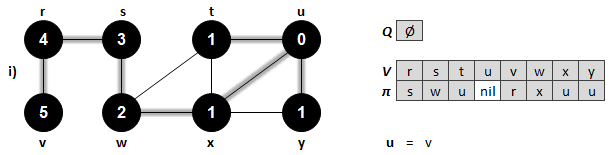
\includegraphics[width=0.8\textwidth]{q7-03.png}
\captionof{figure}{Árvore resultante do algoritmo \proc{BFS}, sendo $s = u$ e a lista de adjacências na ordem $\{x, y, t\}$.}
\label{fig:7.3-1}
\end{center}